\graphicspath{ {HW-PIC/} }


\chapter{Hardware}

    \section{Umsetzung - V1}
    
    \subsection{V1}
        \subsubsection{Versorgung}
        Das Board wird mit 5V über USB-C versorgt, um den ESP32-S3 mit 3V3 zu 
        versorgung, wird ein AMS1117 Spannungswandler verwenden. Dieser wurde ausgewählt, 
        aufgrund der einfachen Implementierung. Die Verluste bei der Umwandlung können vernachlässigt werden, da 
        es sich nicht um ein batteriebetriebenes Gerät handelt.

            \begin{figure}[h]
                \centering
                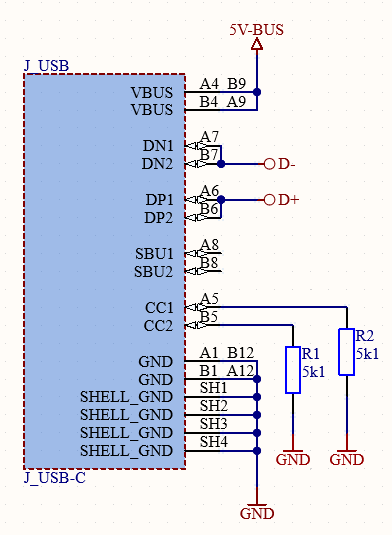
\includegraphics[width=7cm]{usb-c}
                \caption{USB-C Büchse "programmiert" mit Widerständen.}
                \label{fig:sch1}

            \end{figure}

        Die Widerstände R1 und R2 mit 5,1kOhm sind mit den CC-Leitungen auf GND verbunden.
        Dadurch weiß das Netzteil welche Spannung und wie viel Strom es zur verfügung stellen
        muss. 

            \begin{figure}[h]
                \centering
                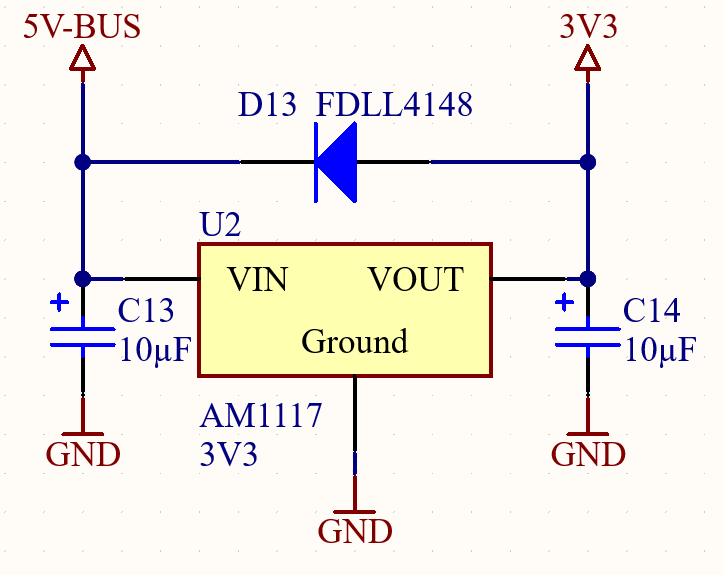
\includegraphics[width=8cm]{powersupply}
                \caption{AMS1117 mit 3V3 Ausgangsspannung.}
                \label{fig:sch2}
                
            \end{figure}

        Ein- und Ausgangsseitig liegt jeweils ein Glättungskondensator. Die Diode wurde hinzugefügt 
        um zu verhindern, dass am Ausgang eine größere Spannung
        anliegt als beim Eingang - wie z.B. beim Abstecken des Gerätes.

        \newpage

        \subsubsection{Mikrocontroller}
        Der ESP32-S3-WROOM-2 ist das Herzstück des Gerätes. Dieser verfügt über eine On-board PCB Antenne
        und kommuniziert darüber mit dem Smart-Home System. 

            \begin{figure}[h!]
                \centering
                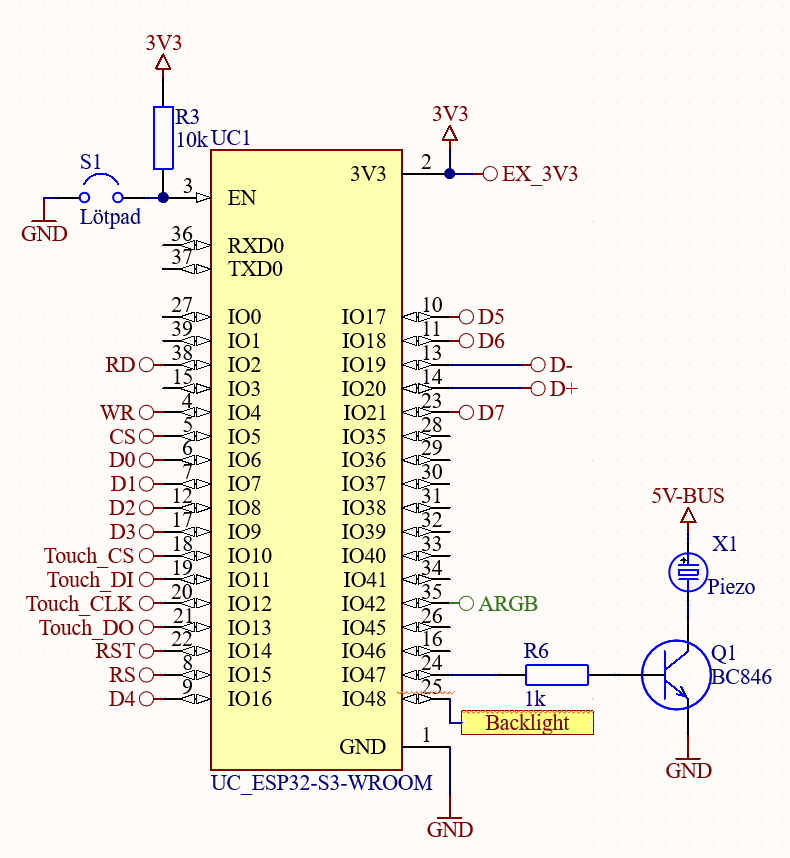
\includegraphics[width=8cm]{microcontroller.png}
                \caption{uC im Schaltplan.}
                \label{fig:sch3}

            \end{figure}

        \subsubsection{Display}
        Das Display wird parallel im 8-BIT Modus angesteuert. Die Pins mit denen 
        kommuniziert wird sind nicht fix in der Libary festgelegt und können am Esp32-S3 
        frei ausgewählt werden. 

            \begin{figure}[h!]
                \centering
                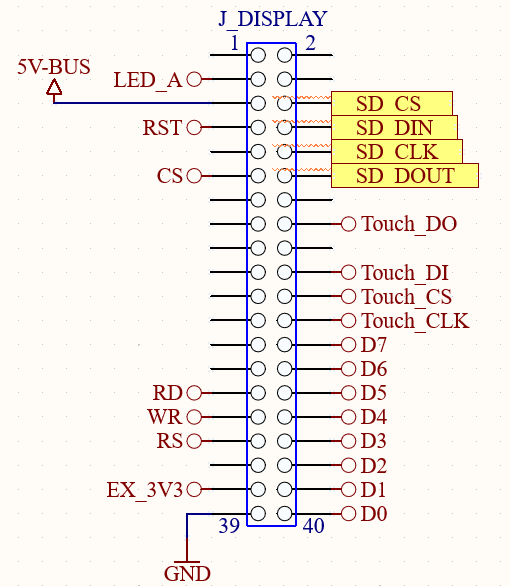
\includegraphics[width=8cm]{connector.png}
                \caption{Stecker für Display und Touch}
                \label{fig:sch4}

            \end{figure}

        Das zugekaufte Display hat ebenfalls einen SD-Kartenleser eingebaut. Dieser wird 
        über SPI ausgelesen(Gelb markiert), ist aber für dieses Projekt nicht in verwendung. 


        \subsubsection{Touch}
        Die Berührung am Resisivtouch-Panel wird vom XPT2046 erfasst und mittels 
        SPI-BUS vom µC ausgelesen. Da es bei der Implementierung von Touch softwareseitig
        Probleme gab, wurde stattdessen ein Drehgeber mit Taste verwendet.
        Dafür wurden die in der Abbildung \ref{fig:sch1} bzw. \ref{fig:sch4} gezeigten Pins mit 
        dem Prefix "Touch" für das Einlesen des Drehgebers verwendet.

        \subsubsection{Rotary Encoder}
        Der Inkrementalgeber hat einen relativen Ausgang mit A und B Signalen. Diese geben beide
        eine definierte Menge Impulse ab. Beide Signale sind zueinander 90° Phasenverschoben. Somit
        kann die Drehrichtung bestimmt werden. 